\documentclass{article}

\usepackage[preprint]{neurips_2020}
% \usepackage[final]{neurips_2020}
% \usepackage[nonatbib]{neurips_2020}
% \usepackage{natbib}
\usepackage[utf8]{inputenc} % allow utf-8 input
\usepackage[T1]{fontenc}    % use 8-bit T1 fonts
\usepackage{hyperref}       % hyperlinks
\usepackage{url}            % simple URL typesetting
\usepackage{booktabs}       % professional-quality tables
\usepackage{amsfonts}       % blackboard math symbols
\usepackage{nicefrac}       % compact symbols for 1/2, etc.
\usepackage{microtype}      % microtypography
\usepackage{graphicx}
% \usepackage{subcaption}
\usepackage{float}

\title{Testing Improvements for Vector Quantized Variational Autoencoders with Novel Data}

\author{
  Shivanshu Gupta
  \And
  Kolby Nottingham
  \And
  Preethi Seshadri
}

\begin{document}

\maketitle

\begin{abstract}
    We explore using the Vector Quantized Variational Autoencoder (VQ-VAE) to generate discrete representations for the Kaokore dataset, which contains images of facial expressions from traditional Japanese illustrations (\url{https://github.com/rois-codh/kaokore}).
    The framework VQ-VAE is built on, Variational Autoencoders (VAE), learns continuous latent representations.
    While continuous representations are flexible, many real world attributes are better defined discretely, and some current state-of-the art model architectures, like transformers, only work with discrete data. 
    In this project, we experiment with VQ-VAEs on a novel dataset and design experiments to better understand the advantages and disadvantages of VQ-VAE and its variant, VQ-VAE2.
    %Since the VQ-VAE paper uses CIFAR10 and 128x128 ImageNet images, there might be additional experimentation and training required to achieve good performance on the Kaokore dataset.
    % VQ-VAEs have been paired with the transformer architecture which, while scalable, can require a lot of compute, so we will experiment with making the method more compute efficient.  % Not sure what to put in this sentence??
    Our results indicate that while the original VQ-VAE algorithm learns faster than its successor, it does not achieve the same level of performance as VQ-VAE2. 
\end{abstract}

\section{Introduction}

Generative machine learning models learn a distribution $p(x,y)$ for data instances $x$ and labels $y$. Compared to discriminative machine learning models that learn $p(y|x)$, generative models can be more difficult to train but come with added benefits. One use case for generative models is mapping data instances to a latent space, which can be used to produce compressed representations as well as to generate new data instances. 

Within the area of generative models, variational autoencoders (VAE) are one of the most well-known and well-studied type of models \cite{VAE}. VAEs use an encoder-decoder architecture, where the encoder compresses the data into a latent space, and the decoder reconstructs the original data from the latent representation. In contrast to standard autoencoders, VAEs are stochastic and have continuous latent representations; the encoder outputs parameters of a probability distribution, and the input to the decoder is sampled from this distribution.

Instead, vector-quantized VAEs (VQ-VAE) learn discrete latent representations \cite{VQ_VAE}. Discrete representations can be advantageous since real world data is often summarized by categorical features. For example, the latent representation for an image containing a discrete set of objects could have discrete latent variables for size, color, orientation, and so on. In fact, VQ-VAEs have been a key component in novel developments such as DALL-E, a model that generates high quality images from text descriptions. At a high level, DALL-E uses a transformer that takes in both the embeddings from text and latent codes from a VQ-VAE trained on images as input \cite{DALLE}.

In this work, we compare VQ-VAE to its variant, VQ-VAE2. VQ-VAE2 builds on VQ-VAE by leveraging a hierarchical structure with a learned prior \cite{VQ_VAE2}. We go into further detail comparing the algorithms in section \ref{methods}. We implement each of these methods and run experiments using the Kaokore dataset. 

\begin{figure}
    \centering
    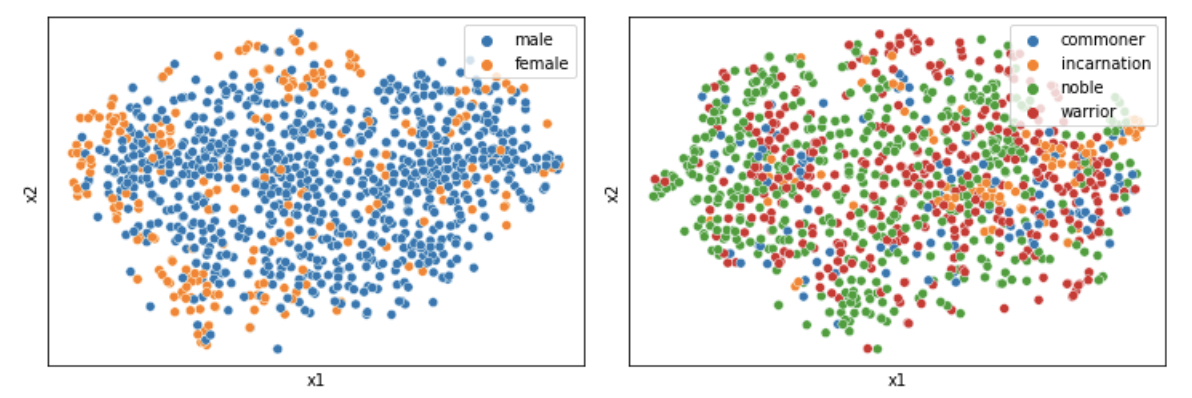
\includegraphics[width=0.7\linewidth]{clustering.png}
    \caption{t-SNE plot for randomly sampled training examples from Kaokore dataset colored by gender and status labels. There are no distinct clusters based on label.}
    \label{fig:clustering}
\end{figure} 

\section{Methods} \label{methods}

In this section, we will describe the various models that are relevant to our work: VAE, VQ-VAE, and VQ-VAE2. While the continuous latent representation of VAEs offers benefits such as latent interpolation, having discrete latent representations can be a more natural fit for certain modalities. Additionally, it has been shown that VAEs can suffer from posterior collapse, a phenomenon in which the learned latent space becomes uninformative. VQ-VAEs have been formulated to address these concerns, while still offering similar performance to VAEs. 

\subsection{VAE}

Similar to vanilla autoencoders, variational autoencoders include an encoder which yields a lower dimensional latent representation and a decoder which reconstructs the input. However, VAEs compute an additional loss term that computes the Kullback-Leibler (KL) divergence between the encoder’s distribution \(q_{\theta}(z|x)\) and \(p(z)\), where \(p(z)\) is typically specified as a normal distribution with zero mean and unit variance. This term serves as a regularizer that keeps similar inputs’ latent representations close together.

% From a generative modeling perspective, imagine data point \textit{i} is sampled by 1) drawing latent variable \(z_{i}\) and 2) drawing data point \(x_{i}\) based on \(z_{i}\). Therefore, we would like to infer a good latent representation \textit{z} given input \textit{x}. This is given by the posterior, \(p(z)\). However, computing the prior, \(p(x)\), requires marginalizing over latents \textit{z} and is often computationally intractable. Instead, variational inference allows us to approximate \textit{p(z|x)} through another distribution \textit{q(z|x)}, which is referred to as the approximate posterior. In other words, we would like to optimize the divergence between the approximate and original posteriors: $\min{KL(q(z|x) \| p(z|x))}$.

The VAE objective function is $\min{KL(q(z|x) \| p(z|x))}$. However, this expression cannot be optimized directly, since it requires computing \textit{p(x)}. While we do not go through the derivation here, minimizing the KL divergence between \textit{q(z|x)} and \textit{p(z|x)} is equivalent to maximizing the evidence lower bound (ELBO), which is computationally tractable. 

\begin{equation}
ELBO = E_{q_{\theta}(z|x)} \log{p_{\phi}(x|z)} - KL(q_{\theta}(z|x)||p(z))
\end{equation}

In practice, VAEs are modeled using neural networks; the approximate posterior is computed from the inference network (encoder) with parameters \(\theta\) and the likelihood is computed from the generative network (decoder) network with parameters \(\phi\). 

\subsection{VQ-VAE}

To learn discrete latent representations, the posterior and prior distributions are categorical instead of gaussian, and samples from these distributions are drawn by indexing an embedding table. The latent embedding space is \(e \in R^{K \times D}\), where \textit{K} is the size of the discrete latent space (i.e., a \textit{K}-way categorical) and \textit{D} is the dimensionality of each latent embedding vector \(e_{i}\).The discrete latent variables \textit{z} are calculated by a nearest neighbor look-up using the embedding table in a process referred to as Vector Quantization (VQ). Therefore, the forward computation pipeline can be viewed as a standard autoencoder with a non-linearity that maps the latents to one of \textit{K} embedding vectors. Since performing a nearest neighbors lookup is non-differentiable, straight-through gradient estimation is used so that the gradient passed back is the same before and after quantization. 

The VQ-VAE loss function consists of three terms: 
\begin{enumerate}
\item Reconstruction loss: Encourages original and reconstructed images to be similar
\item Codebook loss: Encourages the embedding vectors \textit{e} to be close to the encoder output 
\item Commitment loss: Encourages the encoder output to be close to the embedding vectors \textit{e} 
\end{enumerate}

\begin{equation}
L = \log{p(x|z_q(x))} + {\|\textrm{sg}[z_e(x)]-e\|}_{2}^{2} + \beta{\|z_e(x)-\textrm{sg}[e]\|}_{2}^{2}
\end{equation}

The decoder optimizes the first term only, the encoder optimizes the first and last terms, and the embeddings are optimized by the middle term. 

\subsection{VQ-VAE2}

VQ-VAE2 builds on VQ-VAE by using a hierarchical VQ-VAE model to encode images onto a discrete latent space, followed by learning a powerful PixelCNN prior. In this hierarchical architecture, the top-level latent code models global information and the bottom-level latent code, conditioned on the top-level latent, is responsible for representing local details. As a result the learned prior is also hierarchical; the top-level PixelCNN prior is conditioned on the class label, and the bottom level PixelCNN is conditioned on the class label as well as the top-level latent code. The authors show that the VQ-VAE2 framework produces samples that rival the perceptual quality of GANs, while not suffering from lack of diversity. 

\section{Experiments}

\begin{figure}
    \centering
    \includegraphics[width=.9\linewidth]{samples.png}
    \label{fig:samples}
    \caption{The first six rows of images show samples at 1, 12, 14, 16, 18, and 100 epochs for VQ-VAE (left) and VQ-VAE2 (right). The final row shows the corresponding images from the test set.}
\end{figure} 

\begin{table}
    \centering
    \begin{tabular}{c c c}
        & Commitment Loss & Reconstruction Loss \\
        \hline
        VQ-VAE & 0.0793 (0.0027) & 0.0056 (0.0001) \\
        VQ-VAE2 & 0.0025 (0.0035) & 0.0005 (0.0008)
    \end{tabular}
    \label{table:loss}
    \caption{Commitment loss and reconstruction loss on the Kaokore testset for both algorithms. The numbers in paranthesis show standard deviation over three runs.}
\end{table}

\begin{figure}
    \centering
    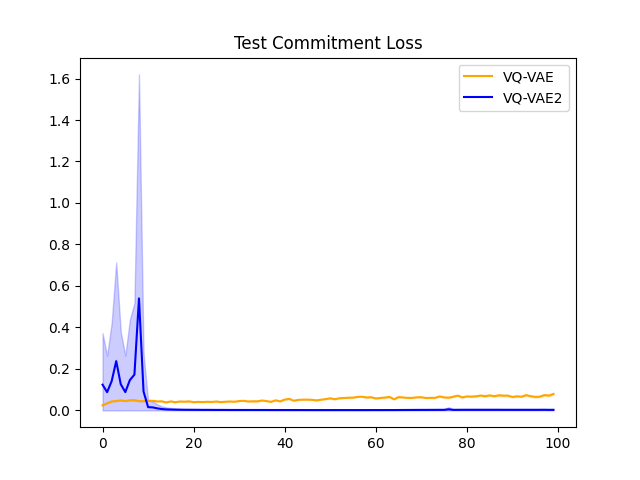
\includegraphics[width=.4\linewidth]{commit.png}
    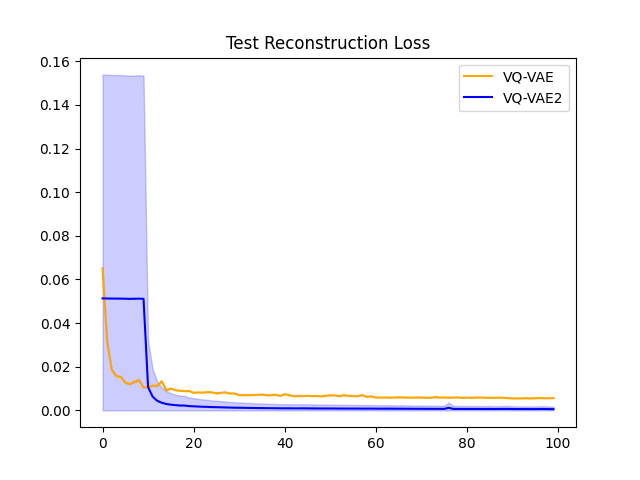
\includegraphics[width=.4\linewidth]{recon.png}
    \caption{Commitment and Reconstruction loss over 100 epochs.}
    \label{fig:loss}
\end{figure}

In a series of experiments, we compare the original VQ-VAE implementation to its variant VQ-VAE2. We use the following implementations as a starting point for VQ-VAE (\url{https://github.com/nadavbh12/VQ-VAE}) and VQ-VAE2 (\url{https://github.com/rosinality/vq-vae-2-pytorch}), and make modifications.

For experimentation, we use the Kaokore dataset consists of facial expressions extracted from pre-modern Japanese artwork \cite{kaokore}. The dataset focuses on cropped face images extracted from Japanese artwork from the Late Muromachi Period (16th century) to the Early Edo Period (17th century) to facilitate research on art history and artistic style. The most recent version contains 8848 colored images, and each image is annotated with gender (male, female) and social status (noble, warrior, incarnation, commoner) labels. WE visualize the data classes in figure \ref{fig:clustering}.

\subsection{Results}

As indicated in table \ref{table:loss} and figure \ref{fig:loss}, the primary advantage of VQ-VAE2 is lower loss. This is achieved due to a better ELBO, coming from the hierarchical model structure. The overall loss is composed of the reconstruction loss plus the commitment loss multiplied by a scalar. This trade-off is the cause of the commitment loss increasing slightly as reconstruction loss lowers. 

Another observation from these results is that VQ-VAE2 starts off training slower than VQ-VAE. Perhaps this initial slowness is the result of training a more complex model. Additional experimentation would be useful to differentiate if this is due to model differences, or other factors like choice of hyperparameters or random seeds. 

This delay in learning can also be seen in figure \ref{fig:samples}. The first row shows that VQ-VAE2 starts off outputting noise for the first few epochs. Rows two through five show samples from the epochs where the loss of VQ-VAE2 changes the fastest. During these epochs, VQ-VAE2 starts to outperform VQ-VAE. Also note that VQ-VAE2 starts to learn lines and image structure before learning colors. It takes about 14 epochs for the model to become more precise in coloring.

\begin{figure}
    \centering
    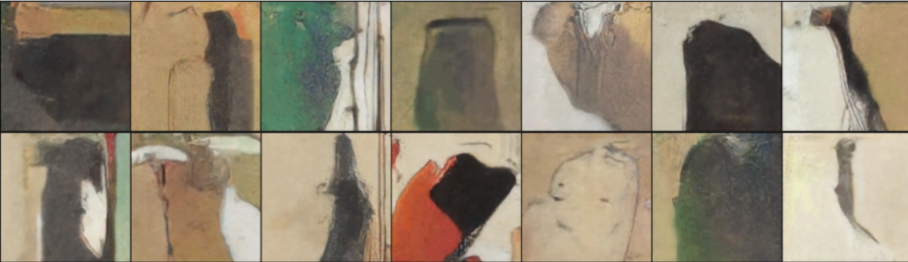
\includegraphics[width=0.7\linewidth]{generations.png}
    \caption{Generated samples using VQ-VAE2 with learned prior}
    \label{fig:generations}
\end{figure}

The VQ-VAE2 authors show that a hierarchical VQ-VAE model augmented with a learned prior over the latent codes is able to generate diverse, high fidelity samples. However, our generated samples in figure \ref{fig:generations} show that generation performance is quite poor, perhaps due to a bug in implementation or not training the model for enough epochs. While the generated samples are stylistically similar to Kaokore instances in terms of color palette and texture, they are unable to capture global information and structure.

\section{Conclusion}

VQ-VAEs have become an increasingly popular type of generative model. The improvements of VQ-VAE2 lower the reconstruction loss of the algorithm, resulting in better overall performance. Our experiments using the recently-constructed Kaokore dataset offer further support to this claim. Additional experimentation is needed to verify whether VQ-VAE2 suffers from slower learning than VQ-VAE across various settings. Furthermore, we need to spend more time understanding why image generation is poor using VQ-VAE2 with the PixelCNN prior, since this has been used in previous work to generate high fidelity images. 

% TODO add bibliography
\bibliographystyle{plain}
\bibliography{neurips_2020}

\end{document}